% ==================================================
% Appendix: Printable plots %
% ==================================================

\chapter[Printable plots]{Printable plots}
\label{appendix:print}
% Edit count: 0

\begin{figure}
    \centering
    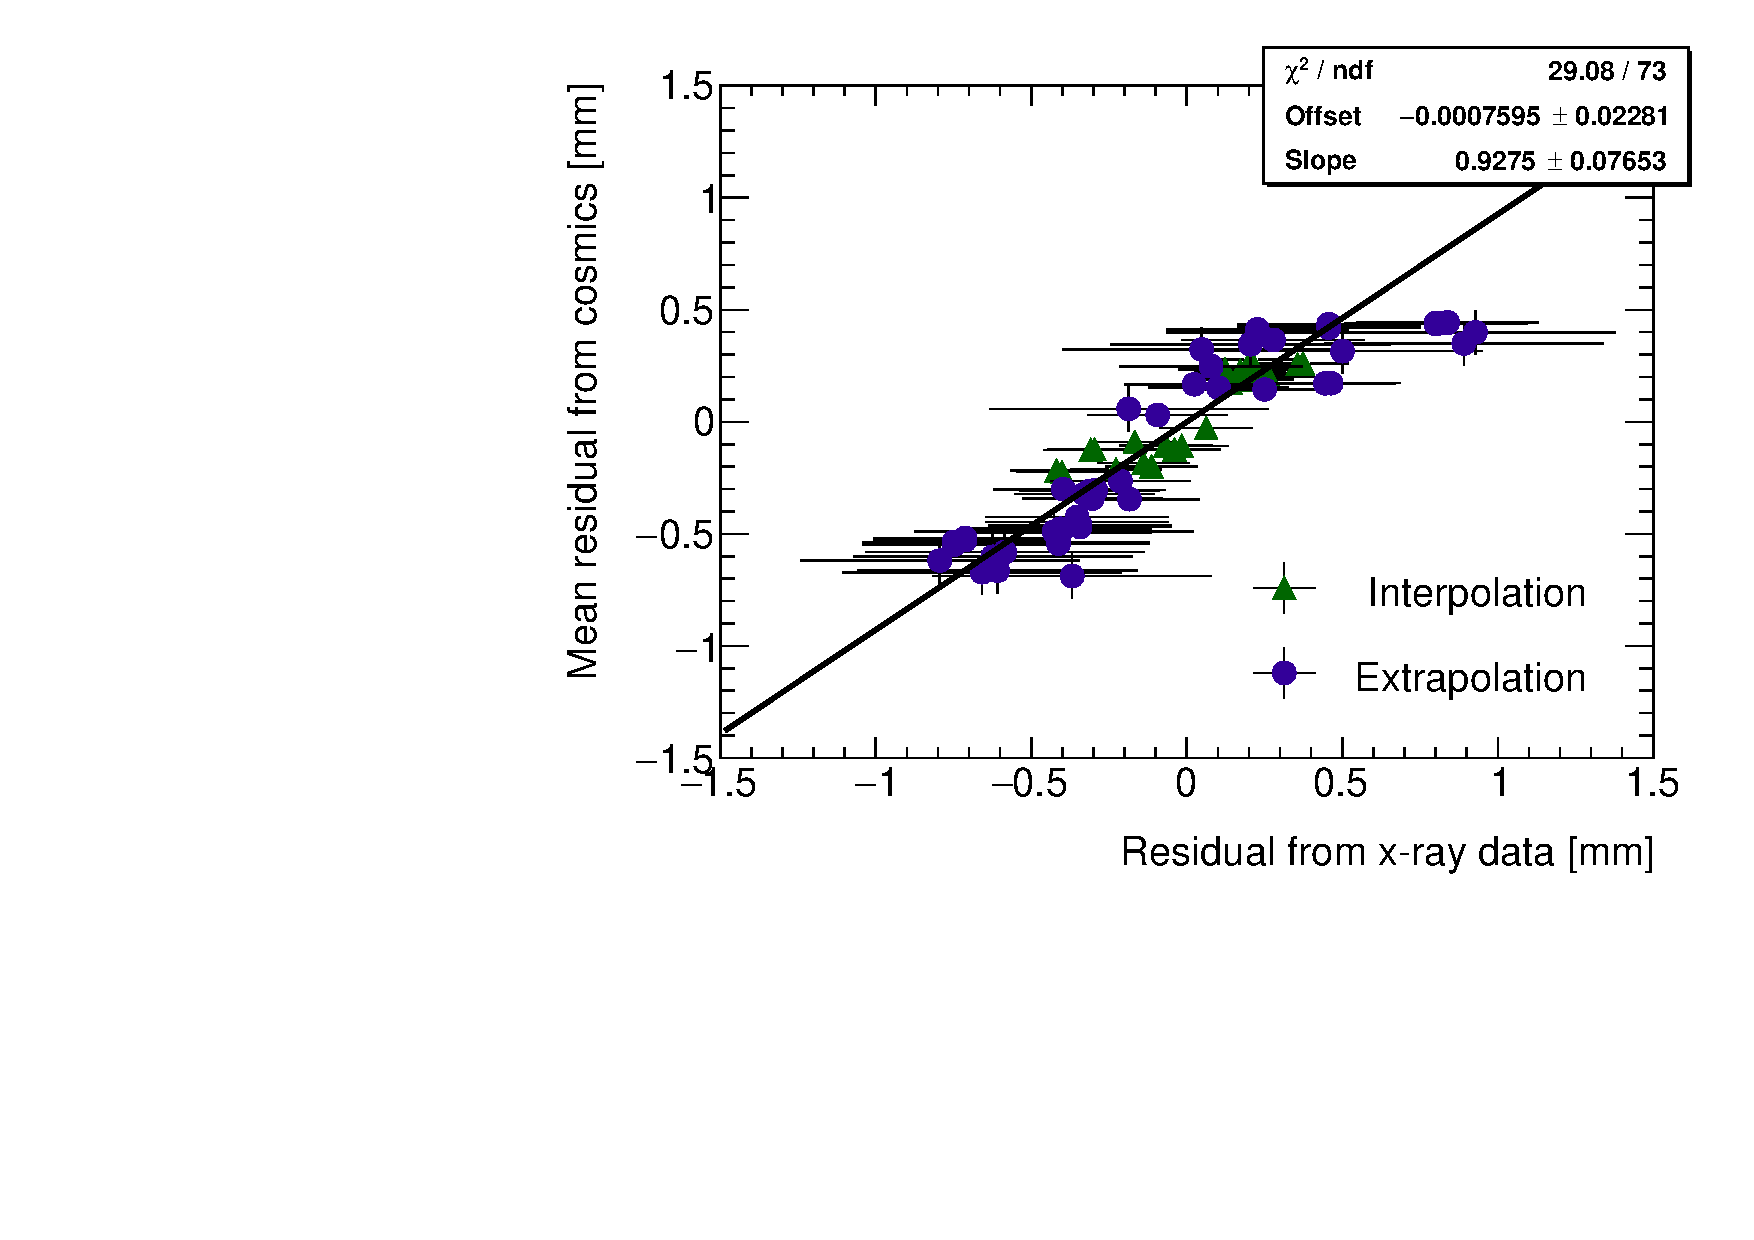
\includegraphics[width = \textwidth]{figures/figure_QL2P11_3100V_2021-08-05_QL2P11_local_cosmic_and_xray_data_correlation_plot_printable.pdf}
    \caption{Correlation plot between x-ray and cosmics residuals for all tracking combinations for QL2.P.11. Each rectangle is centered on an x-ray and mean cosmics residual pair. The width of the rectangles in $x$ and $y$ are the uncertainty in the x-ray and mean cosmics residual respectively. A printable version of figure~\ref{fig:correlation} in section~\ref{sec:assessing_correlation}.}
    \label{fig:correlation_print}
\end{figure}

\begin{figure}
    \centering
    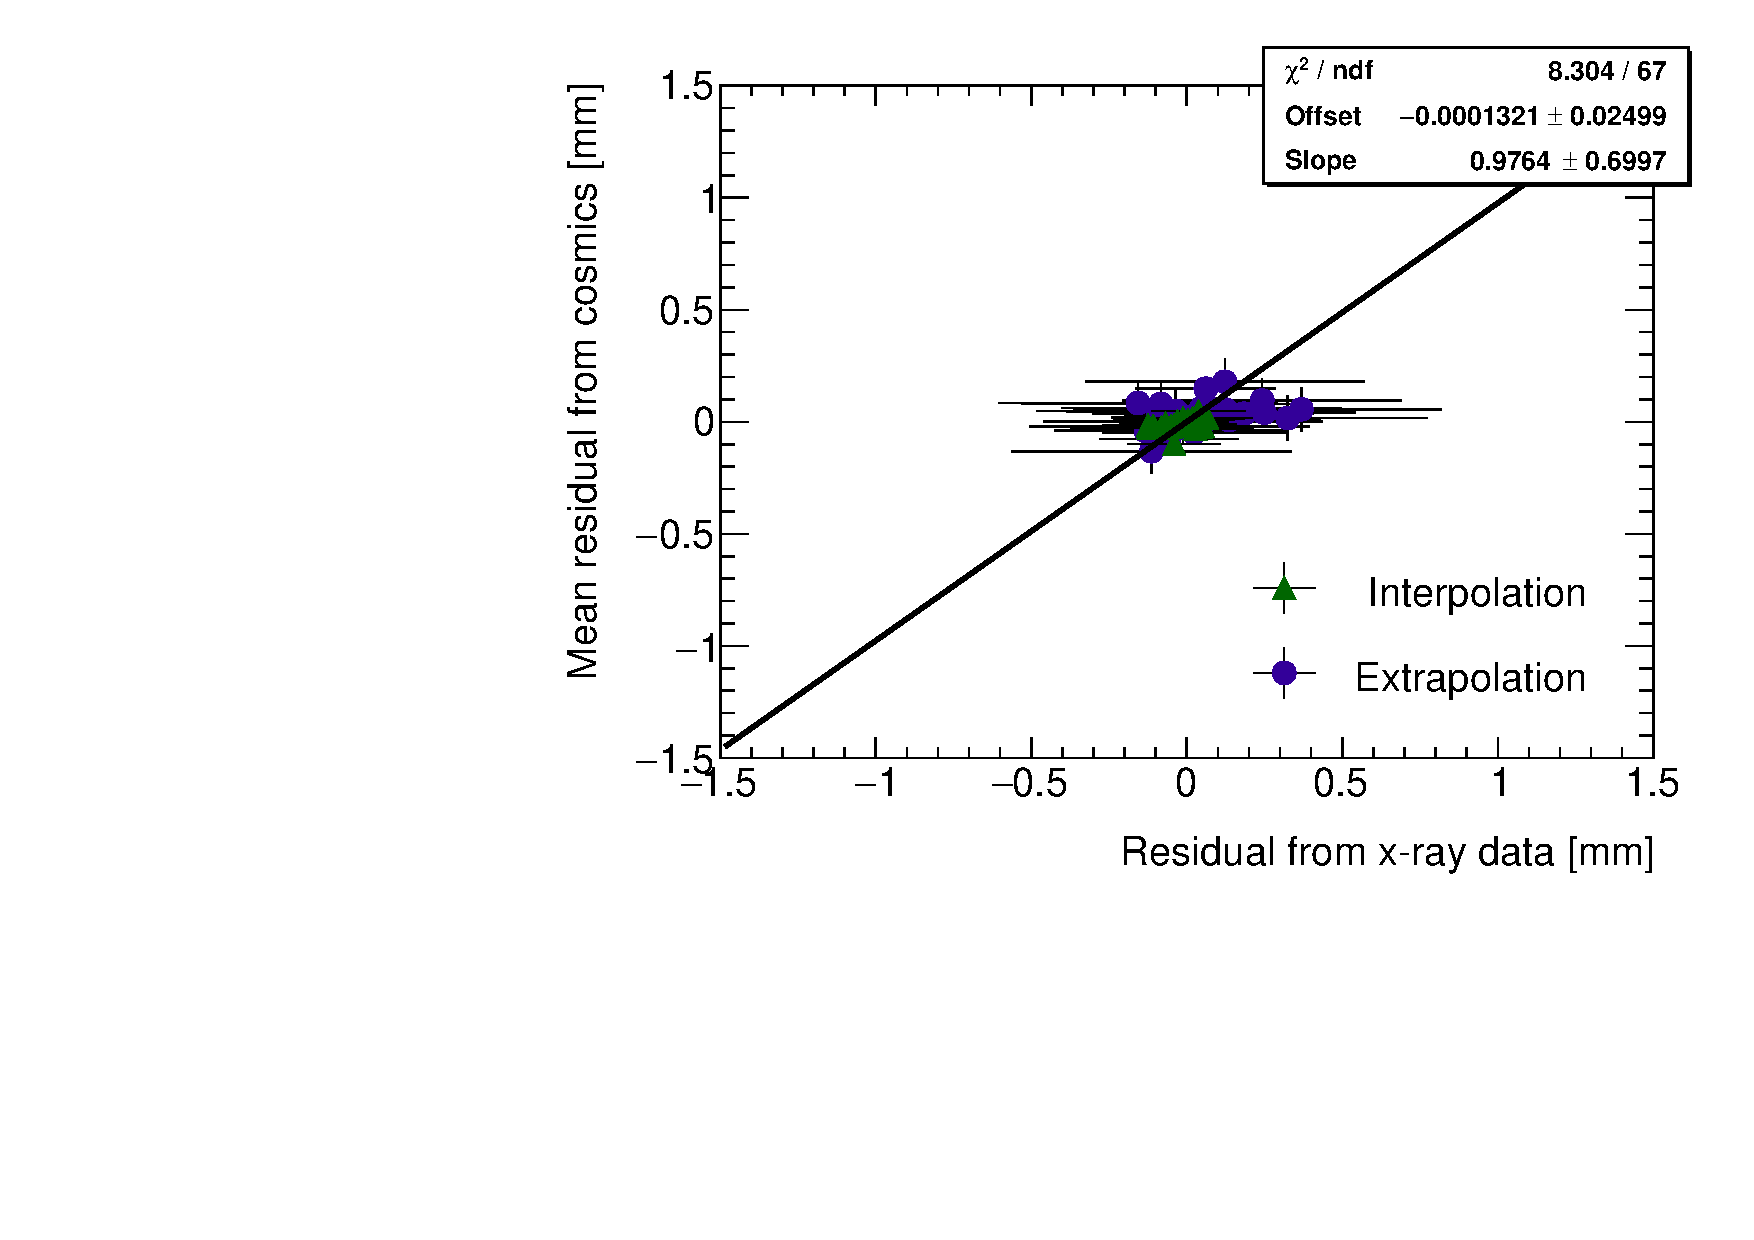
\includegraphics[width = \textwidth]{figures/figure_QL2P08_3100V_2021-08-16_QL2P08_local_cosmic_and_xray_data_correlation_plot_printable.pdf}
    \caption{Correlation plot between x-ray and cosmics residuals for all tracking combinations for QL2.P.8. Each rectangle is centered on an x-ray and mean cosmics residual pair. The width of the rectangles in $x$ and $y$ are the uncertainty in the x-ray and mean cosmics residual respectively. A printer friendly version of this plot is available. A printable version of figure~\ref{fig:no_correlation} in section~\ref{sec:assessing_correlation}.}
    \label{fig:no_correlation_print}
\end{figure}